\documentclass[a4paper]{article}
\usepackage[utf8]{inputenc}
\usepackage[spanish, es-tabla, es-noshorthands]{babel}
\usepackage[table,xcdraw]{xcolor}
\usepackage[a4paper, footnotesep = 1cm, width=20cm, top=2.5cm, height=25cm, textwidth=18cm, textheight=25cm]{geometry}
%\geometry{showframe}

\usepackage{tikz}
\usepackage{amsmath}
\usepackage{amsfonts}
\usepackage{amssymb}
\usepackage{float}
\usepackage{graphicx}
\usepackage{caption}
\usepackage{subcaption}
\usepackage{multicol}
\usepackage{multirow}
\setlength{\doublerulesep}{\arrayrulewidth}
\usepackage{booktabs}
\usepackage{mathrsfs,amsmath}
\usepackage{hyperref}
\hypersetup{
    colorlinks=true,
    linkcolor=blue,
    filecolor=magenta,      
    urlcolor=blue,
    citecolor=blue,    
}

\newcommand{\quotes}[1]{``#1''}
\usepackage{array}
\newcolumntype{C}[1]{>{\centering\let\newline\\\arraybackslash\hspace{0pt}}m{#1}}
\usepackage[american]{circuitikz}
\usetikzlibrary{calc}
\usepackage{fancyhdr}
\usepackage{units} 

\graphicspath{./Imagenes}

\pagestyle{fancy}
\fancyhf{}
\lhead{22.05 ASSD}
\rhead{Mechoulam, Lambertucci, Rodriguez, Londero}
\rfoot{Página \thepage}

\begin{document}

\subsection{Conversor Sigma Delta $\Sigma \Delta$}

\subsubsection{Introducción}
El conversor sigma-delta o delta-sigma según la literatura consultada, tuvo su aparición durante los años 60's y 70's. Aunque su nombre pueda sugerir un tipo de tecnología muy compleaja la realidad es que no lo es en términos constructivos. Los moduladores sigma-delta nos permiten alcanzar una digitalización de alta resolución (16bits o 24bits) sin la necesidad de utilizar ADC de ese porte. Esto se consigue dado que este diseño permite alcanzar un nivel de ruido de cuantización equivalente a la de un ADC de mayor porte utilizando un ADC más modesto.


\subsubsection{Arquitectura}

A continuación presentamos la topología implementada:

\begin{figure}[H]
	\centering
	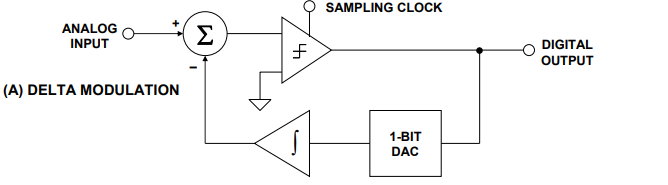
\includegraphics[width=0.7\linewidth]{ImagenesEjercicio2/diagramaEnBloques}
	\caption{Modulador $\Sigma\Delta$ de primer orden}
	\label{fig:diagramaenbloques}
\end{figure}

Como se puede observar el modulador $\Sigma\Delta$ se basa en un circuito con un solo camino de realimentación negativa que incorpora un un cuantificador y un DAC en su interior.



\subsubsection{Modulador}
La salida del modulador $\Sigma\Delta$ es un bit-stream de valores binario arbitrarios. En esta secuencia se encuentra codificada toda la información necesaria para poder reconstruir la señal original. Aún más importante que reconstruir la señal original, es conseguir un valor preciso de la misma en un instante de tiempo. Es decir, poder tomar mediciones. Este tipo de conversores son famosos por la alta resolución que son capaces de proveer. Sin embargo, el limite de su funcionalidad aparece cuando se los quiere utilizar en un ambiente donde la señales cambian de forma abrupta.

\begin{figure}[H]
	\centering
	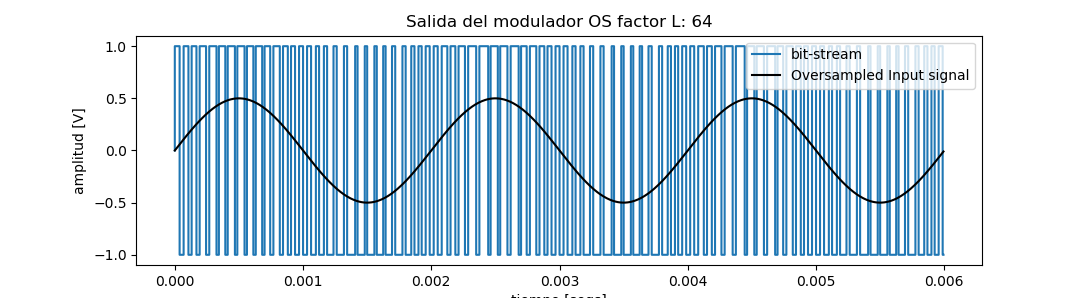
\includegraphics[width=0.7\linewidth]{ImagenesEjercicio2/BitsStream64}
	\caption{}
	\label{fig:bitsstream64}
\end{figure}







\subsubsection{Demodulador}

\subsubsection{Noise Shaping}
Una de las más notables características de este tipo de modulación es el efecto llamado \textbf{noise-shaping}.

\begin{figure}[H]
	\centering
	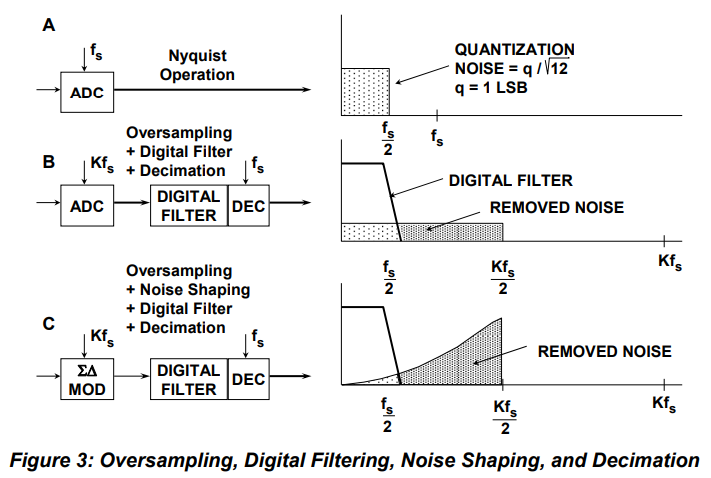
\includegraphics[width=0.7\linewidth]{ImagenesEjercicio2/NoiseShappingAN}
	\caption{}
	\label{fig:noiseshappingan}
\end{figure}


\subsubsection{Simulación de aplicación real}
En este ejemplo vamos a simular la digitalización de una conversación, la voz humana... rango audible de ... por lo tanto es 

\subsubsection{Ejemplos varios}

\end{document}